\documentclass[a4paper,12pt]{article}

% Pakiety potrzebne do koloru tła i tekstu
\usepackage[utf8]{inputenc}
\usepackage[T1]{fontenc}
\usepackage{lmodern}
\usepackage{xcolor}
\usepackage{pagecolor}
\usepackage{titling}
\usepackage{datetime2}
\usepackage{lmodern}
\usepackage{graphicx}
\usepackage{float} % dodaj w preambule!
\usepackage{amsmath}

% Czarny motyw
\definecolor{bgcolor}{RGB}{23, 23, 23}
\definecolor{textcolor}{RGB}{255, 174, 69}
\pagecolor{bgcolor}
\color{white}

% Dane do tytułu
\title{SISE - notatki pod egzamin}
\author{Dawid Gradowski \\ \texttt{@puckmoment} na dc}
\date{15.06.2025}

\begin{document}

% Strona tytułowa
\maketitle
\thispagestyle{empty}
\newpage
\tableofcontents
\newpage

% Tu zaczyna się treść notatek
\section*{Wstęp}
Notatki na podstawie pytań, które wpadły mi w ręce. Nie jestem autorem wszystkich tekstów jakie zostaną tu umieszczone.
\section{Co to jest sztuczna inteligencja?}
Jest to imitacja inteligencji człowieka realizowana przez maszyny,
pozwalająca im na wykorzystanie wrodzonej i zdobytej wiedzy do
rozwiązywania nowych problemów 

\section{Co to jest zmienna lingwistyczna?}
Zmienna lingwistyczna to zmienna, której wartościami są słowa lub wyrażenia języka naturalnego, a nie konkretne liczby.

Weźmy na przykład zmienną lingwistyczną „temperatura”. Zamiast przyjmować wartości liczbowe (np. 20°C, 30°C), może przyjmować wartości takie jak:
\begin{itemize}
    \item zimno
    \item chłodno
    \item ciepło
    \item gorąco
\end{itemize}
Każda z tych wartości lingwistycznych może być dalej modelowana za pomocą zbiorów rozmytych – np. „ciepło” może obejmować temperatury od 20°C do 30°C, ale z różnym stopniem przynależności (np. 22°C to „trochę ciepło”, 28°C to „bardzo ciepło”).
\newpage
\section{Czym jest funkcja aktywacji, jaka jest najczęściej stosowana?}
Funkcja aktywacji to pojęcie używane w sztucznej inteligencji do
określenia funkcji, według której obliczana jest wartość wyjścia
neuronów sieci neuronowej.

Najczęściej używana jest sigmoida:
\[
    y = \frac{1}{1+\exp(-\beta s)}
\]
w której 
\begin{itemize}
    \item $\beta$ - wybiera użytkownik, wpływa na kształt wykresy, wzrost $\beta$ $\to$ większy kąt
    \item $s$ - sygnał
\end{itemize}

\section{Co to są sieci neuronowe, do czego służą?}
Sieciami neuronowymi nazywamy system którego budowa i zasada
działania w pewnym stopniu wzorowana jest na funkcjonowaniu
fragmentów rzeczywistego systemu nerwowego. Na przesłankach
biologicznych oparte są schematy sztucznych neuronów wchodzących w
skład sieci oraz jej struktura.

Służą do uczenia maszynowego, by maszyna mogła rozwiązywać nowe
problemy, których nigdy nie widziała na podstawie wiedzy zdobytej
podczas uczenia.

\section{Dlaczego neurony nazywamy neuronami?}
Sztuczne neurony które są w sieciach neuronowych są zbudowane na
podobieństwo neuronów jako komórek nerwowych. Mają wejścia, coś co
przetwarza i wyjścia.

\section{Co to dane i informacje, różnice między nimi?}
Dane zawsze reprezentują fakty, bez odpowiedniej interpretacji nic nie
znaczą. Dopiero informacja co oznaczają te dane pozwala nam
zrozumieć ich sens.

\section{Wzór na zbiór rozmyty?}
Zbiór par składający się z poszczególnych elementów przestrzeni
rozważań i ich stopni przynależności do tego zbioru rozmytego. 

Zbiory rozmyte (fuzzy) zawierają obiekty zpełniające nieprecyzyjne własności przynależności;
innymi złowy przynależność może być w pewien sposób przybliżona.

Zbiór rozmyty $A$ w pewnej przestrzeni rozważań $X = {x}$ określa się jako zbiór par
\[
    A = {(x, \mu_A(x))}
\]
gdzie \break $\mu_A: X \to [0, 1]$ jest funkcją przynależności zbioru rozmytego $A$,
a wartość $\mu_A \in [0, 1]$ jest stopniem przynależności elementu $x \in X$ do zbioru
rozmytego $A$

Znaczy to mniej więcej tyle, że zamiast przynależności pełnej "tak"(1) i "nie"(0) jak w 
zbiorach klasycznych, mogą być to wartości stopnia przynależności od 0 do 1.

\section{Gdzie był wykorzystany perceptron, co to perceptron?}
Jest to najprostsza sieć neuronowa, składająca się z jednego bądź wielu
niezależnych neuronów. Przeznaczeniem było rozpoznawanie znaków
alfanumerycznych. Innowacją było tu zastosowanie procesu uczenia jako
metody programowania systemu.

\section{Perceptron wielowarstwowy}
Może mieć 3 warstwy:
\begin{itemize}
    \item Wejściową (linową),
    \item ukrytą (nieliniową),
    \item wyjściową (liniową).
\end{itemize}
Może mieć więcej warstw ale nie ma to sensu. 
\section{Czym jest wyostrzanie?}
wyostrzanie (defuzzyfication) jest przekształceniem, dzięki któremu zbiór rozmyty
$B$ zostaje zastąpiony przez pojedyńczą liczbe $\bar{y} \in Y$ będącą jesgo reprezentacją.
Intuicja podpowiada, że wyostrzanie powinno być rodzajem uśredniania. Oto kilka popularnych metod.

Metoda środka ciężkości (cog - center of gravity) jest znanym z fizyki rachunkiem, w którym masa (lub ciężar) jest
zastępowana przez wartości funkji przynależności.
Dla ciągłych funkcji przynależności mamy:
\[
    \bar{y} = cog(B) = \frac{\int\limits_A{\mu_B (y)y} \cdot dy}{\int\limits_A{\mu_B (y)} \cdot dy}
\]

\section{Wykresy wyostrzenia?}
\begin{figure}[H]
    \centering
    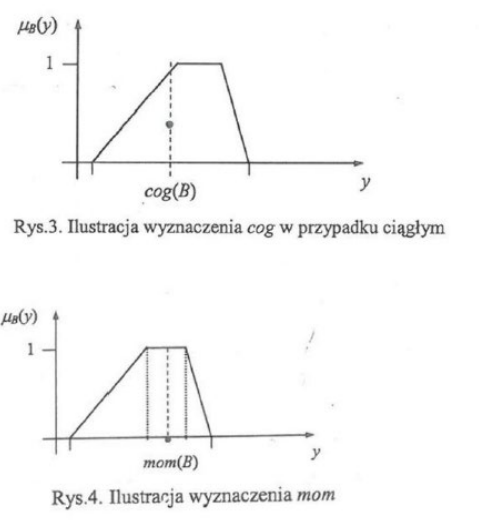
\includegraphics[width=0.85\textwidth]{img/Wykresy.png}
    \label{fig:moj_obrazek}
\end{figure}
\newpage
\section{Czym jest Adaline?}
Adaline jest to adaptacyjny liniowy neuron (Adaptive Linear Neuron). Jego wagi mogą ulegać
zmianie. Ma generować odpowiednie wyjście dla określonych wejść.
\[
    o = \sum_{j = 1}^{n}w_j x_j = w^T x
\]
Nauka odbywa się w procesie nadzorowanym z tzw. nauczycielem. Od wymaganej odpowiedzi \textbf{$r$} (właściwe rozwiązanie)
odejmujemy \textbf{$o$} (wyjście) i otrzymujemy \textbf{$d$}. Otrzymana wartość potrzebna jest w regule Delta - czyli zmiany wagi
w oparciu o \textbf{$d$}.

Reguła Delta ($\Delta$):
\[
    w^{k + 1} = w^k + \eta dx
\]
\[
    d = r - o
\]
gdzie
\begin{itemize}
    \item $r$ - wartość oczekiwana
    \item $o$ - aktualna warotść na wyjściu
\end{itemize}
\begin{figure}[H]
    \centering
    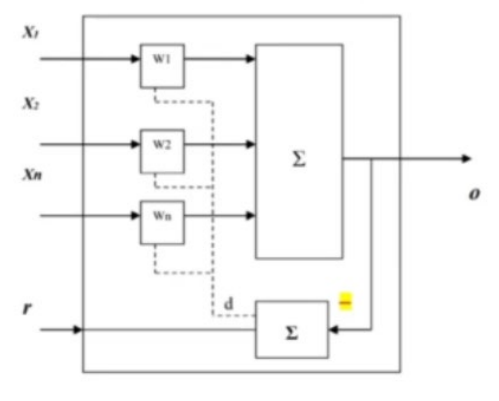
\includegraphics[width=0.8\textwidth]{img/adaline.png}
    \label{fig:moj_obrazek}
\end{figure}
\newpage
\newpage
\section{Uczenie Adaline}
Uczenie Adaline jest oparte o Regułe Delta ($\Delta$):
\[
    w^{k + 1} = w^k + \eta dx
\]
\[
    d = r - o
\]
gdzie
\begin{itemize}
    \item $r$ - wartość oczekiwana (cel)
    \item $o$ - aktualna warotść na wyjściu
\end{itemize}

Interpretacja tej reguły:

Niech $d > 0$, tzn. $r > o$.
Oznacza to, że sygnał wyjściowy z neuronu jest za mały.


sygnał wyjściowy zależy od kąta pomiędzy wektorami x i w; kąt jest za duży.
\[
    o = \sum w_i x_i = w^T x \Leftarrow \text{iloczyn skalarny}
\]
Jeśli $x$ i $w$ są znormalizowane, tzn. $||x|| = x^T x = ||w||=w^T w = 1$, to 
$o = \cos \alpha$, gdzie kąt $\alpha$ jest kątem między wektorami $x$ i $w$.

Należy uzgodnić kierunki $x$ i $w$. Dodając wektororwo $x$ od wektgora $w$, otrzymuje się nowy wektor 
$w^{k + 1}$ bardziej zgodny z $r$ niż poprzedni.

Ponieważ zwykle $\eta d < 1$, to wg wzoru ($\Delta$) dodaje sie tylko fragment wektora $x$, co zapobiega
zbyt gwałtownym obrotom wektora $w$.

Gdy $d < 0$, tzn. $r < o$, następuje oddalanie wektorów $x$ i $w$; odpowiedź była zbyt silna.

\section{Czym jest Madaline?}
Madaline (Multiple ADAptive LINear Elements) to sieć neuronowa zbudowana z wielu adaptacyjnych neuronów liniowych (ADALINE), które tworzą jedną lub więcej warstw.
Każdy neuron otrzymuje wszystkie dane wejściowe i dokonuje liniowej kombinacji wag oraz sygnałów wejściowych, a następnie stosuje funkcję progową.
Dzięki odpowiedniej organizacji neuronów i zasadzie głosowania, sieć może rozpoznawać także funkcje nieliniowe.
W niektórych przypadkach struktura może zawierać więcej neuronów niż jest to konieczne do realizacji danego zadania, co czyni ją potencjalnie nadmiarową.

\section{Jaki wzór sugerował zamiast sigmoidalnej? – tangens hiperboliczny}
Tangens hiperboliczny:
\[
    \text{tgh }x = \frac{\sinh x}{\cosh x} = \frac{e^x - e^{-x}}{e^x + e^{-x}}
\]
może być również oznaczone jako $\tanh x$ i $\text{th }x$.

\section{Sieć Kohonena}
Jest to najbardziej znana i najczęściej stosowana sieć samoucząca się,
realizuje zasadę samoorganizacji (SOM). Jest to także najbardziej znany
przykład sieci konkurencyjnej wykorzystującej koncepcje sąsiedztwa. W
wyniku uczenia tej sieci powstaje mapa topologiczna, której aprioryczna
interpretacja jest niemożliwa (bo sieć uczy się bez nauczyciela i
użytkownik nie ma kontroli nad tym co sieć robi). Jednak po nauczeniu
można zwykle ustalić, jakie znaczenie mają poszczególne rejony tej mapy
(tworzonej przez sygnały wyjściowe pochodzące z warstwy
topologicznej) na podstawie analizy konkretnych danych wejściowych.

Klasycznie: Sieć wybiera neuron o najwyższym poziomie aktywacji i w ten sposób oeklaruje go jako zwycięzce.
Zwycięzka bierze wszystko (w literaturze ang.: winner takes all).

Tym samym sieć jest \textbf{klasyfikatorem}.

Liczba neuronów liniowych wyznacza liczbę klas, które potencjalnie sieć może rozróżniać.
Elementami wektora wejść $x$ są cechy na podstawie których rozróznia się klasy.

CEL NAUKI: $w_i ^{p*(k + 1)} \sim x_i^{(k)}$

Dodatkowe pytania:
\begin{itemize}
    \item {Ile ma warstw kohonen? (1)}
    \item {Może mieć więcej? ( nie )}
    \item {Dlaczego? ( bo założenie funkcji liniowych nadal jest liniowe wiec nie ma sensu)}
\end{itemize}

\subsection{Kohonen – winner takes all (wzór)}
\[
    w_i^{p(k+1)} = w_i^{p(k)} + \eta^{(k)} (x_i^{(k)} - w_i^{p(k)})
\]
gdzie:
\begin{itemize}
    \item $w$ - wektor wag
    \item $x$ - wejście
    \item $\eta$ - współczynnik kroku
    \item $p$ - pokazuje, że to zwycięzca
\end{itemize}

\subsection{Modyfikacja na winner takes most (dopisanie * odległość od sąsiadów)}
Chuj wie :)


\section{Przeuczenie w wielowarstwowym perceptronie?}

\section{Algorytm genetyczny}

\section{Operacje genetyczne}

\section{Czym jest ruletka?}
\subsection{Wzór na wycinek?}

\section{Gwiazda wejść/wyjść?}

\section{Uczenie nadzorowane?}

\section{Metoda gradientowa?}

\section{Notacja wektorowa(Diraca)?}

\section{Funkcja celu}

\section{Momentum i alpha}

\section{Gaz neuronowy}

\end{document}